\chapter{Model Application}
\label{chp:chapter4}
\graphicspath{{figures/}{figures/chapter4/}}

\section{Overview}
In this chapter, we summarize the methodology used to identify vulnerable
links on Utah’s highway network. We also apply the model to scenarios
where critical highway links are removed from the model network. This
includes first a detailed analysis of a single scenario, where I-80
between Salt Lake and Tooele Counties is severed. We compare the model
output to an alternative method that measures only the change in travel
time and does not allow for mode or destination choice. The model was then
applied to 41 individual link closure scenarios throughout the state.

\section{Vulnerable Link Identification}

Two methodologies were developed to identify vulnerable network links in
Utah. The first method resembles the process used by AEM to determine
threat categories, and threat proximity thresholds to highway links. This
methodology was ultimately not used in the resiliency model due to its
complicated nature which involved identifying multiple risk factors. The
second method uses an online Risk Priority Analysis map created by UDOT
combined with familiar knowledge of Utah’s road system. Using this second
method, links were identified due to their location in relation to
populations or geography. Many were suspected choke points or were points
of interest to the BYU team or UDOT officials.

\section{Single Scenario Analysis}

This section outlines an in-depth analysis that was conducted to ensure
the resiliency model was accurately capturing trips with OD pairs in the
targeted area around a closed link (in an urban area, most trips would be
generated or terminate in areas directly adjacent to the broken link).
This analysis was done on a link between Tooele and Salt Lake City, Utah.

Scenario 50, located along I-80 between Tooele and Salt Lake Counties, was
examined to ensure the resiliency model was capturing trips in the
vicinity of a broken link. Analyzing the model outputs at a localized
level was necessary to ensure that the model was appropriately estimating
trips and capturing them in the areas that were expected. In scenario 50,
if many effected trips had not been originated or terminated in Tooele and
Salt Lake counties, that would have signaled that a problem was present in
the model. This localized analysis shows that a broken link mainly effects
the area surrounding that link, and the key takeaway here is that the
model functions as intended.

Another method we used to estimate trip costs is the travel time method,
which serves to capture trips that have fixed OD pairs such as freight and
recreational trips. This localized analysis also looks at this method.

Table \ref{tab:tooeletable} compares the overall costs between the logsum and travel
time methods, the specific cost for trips originating in Tooele and ending in Salt
Lake and includes a trip comparison as well. From Table \ref{tab:tooeletable}, we can
see that the logsum method captures about \$53,897 in experienced expense due to the
closure of the link. Specifically, between Tooele and SLC, the logsum based
resiliency model captures \$20,746 of expense, which is approximately 51.89\% of the
total expense as seen in Table \ref{tab:tooeletable2}. This shows that the resiliency
model is effectively capturing trips in the correct areas based on the percent
comparison capture rate in Table \ref{tab:tooeletable2}. When we look at the travel
time method of analysis, we can see that the costs at both the local and statewide
levels are much greater with \$437,401 and \$406,899 respectively estimated as the
costs due to just the increase in travel time, not using the logit-based model.

\begin{table}

\caption{\label{tab:tooeletable}Tooele Table}
\centering
\begin{tabular}[t]{lllllll}
\toprule
...1 & Total Overall Costs & ...3 & Tooele - SLC Cost & ...5 & Base Trips
& ...7\\
\midrule
Purpose & Logsum & Travel Time & Logsum & Travel Time & Tooele - SLC &
Whole Network\\
HBW & \$15397.06 & \$244275.72 & \$12143.11 & \$233373.56 & 7980 & 1684141\\
HBO & \$12882.89 & \$108412.94 & \$3577.62 & \$98163.53 & 6665.86 & 4593248\\
NHB & \$25635.92 & \$84712.36 & \$5025.24 & \$75361.98 & 1025
& 2611185\\
REC & \$398.72 & \$398.72 & \$40.73 & \$40.73 & 3 & 2385\\
\addlinespace
XXP & \$3690.26 & \$55870.17 & \$55870.17 & \- & 0 & 22350\\
Freight & \$911254.89 & \$10883835.01 & \$111772.5 & \$111772.5 & 515811 &
875183\\
Total Logsum & \$53897.87 & \$437401.02 & \$20745.97 & \$406899.06 &
15672 & 8888574\\
Total & \$969241.74 & \$437401.02 & \$132559.20 & \$406899.06 & 531486 & 9788493\\
\bottomrule
\end{tabular}
\end{table}

\begin{table}

\caption{\label{tab:tooeletable2}Tooele Table Again}
\centering
\begin{tabular}[t]{llrr}
\toprule
Logsum / Base & ...2 & Logsum / Tooele - SLC Logsum & Travel Time / Tooele
- SLC Travel Time\\
\midrule
 &  &  & \\
All Trips & Tooele - SLC &  & \\
0.0630 & 0.0342 & 0.5189 & 0.9554\\
0.1188 & 0.0679 & 0.5174 & 0.9055\\
0.3026 & 0.0136 & 0.0400 & 0.8896\\
\bottomrule
\end{tabular}
\end{table}

The logsum and travel time methods can be broken down into the overall costs and the
comparable costs. The comparable costs are made up of those purposes which are
included in both the resileincy model and in the travel time method for determining
cost. HBW, HBO, and NHB trip purposes can be compared because all three trip purposes
are represented by each method of cost estimation.

The travel time method measures the difference in travel time between the base
scenario and any other scenario caused by link closure, and then multiplies that
difference by the VOT for each trip purpose and the number of trips estimated for
each trip purpose. For external trips, freight trips, and REC trips, these were all
extracted directly from USTM. Attempting to include a calculation of the costs
associated with increased travel time for freight trips, external trips, and REC
trips allows a better estimation of the true cost experienced by all road users, not
just those who areincluded in the resiliency model.

The HBW, HBO, and NHB purposes are also estimated using the logsum model. Calculating
the costs associated with the change in logsum provides a more precise and accurate
estimate of the costs experienced by these users due to link loss. Ultimately, the
logit-based model is more sensitive to changes in the network for those purposes
which are included in the resiliency model, but a way to account for all purposes
must be developed as well. Thus, by combining elements from the travel time method
and the resileincy model, an estimate can be made that represents all traffic on the
USTM network.

\section{Comparative Scenario Results}

We now apply the model to compare 40 additional scenarios where individual highway
facilities are removed from the model highway network. These scenario locations are
shown in Figure \ref{fig:linksmap}, and were identified in a report by \cite{aem2017} and the research team. AEM approached
the idea of systemic resiliency by attempting to classify various types of threats
toward specific infrastructure types. This method, while valid, was difficult to
implement statewide. Some facilities have obvious natural threats such as earthquake,
flood, or landslide, or are natural choke points on the USTM network. Because of the difficulty
associated with identifying links in a similar method to AEM, the BYU team identified links using UDOTs risk analysis tool.

\begin{figure}

{\centering 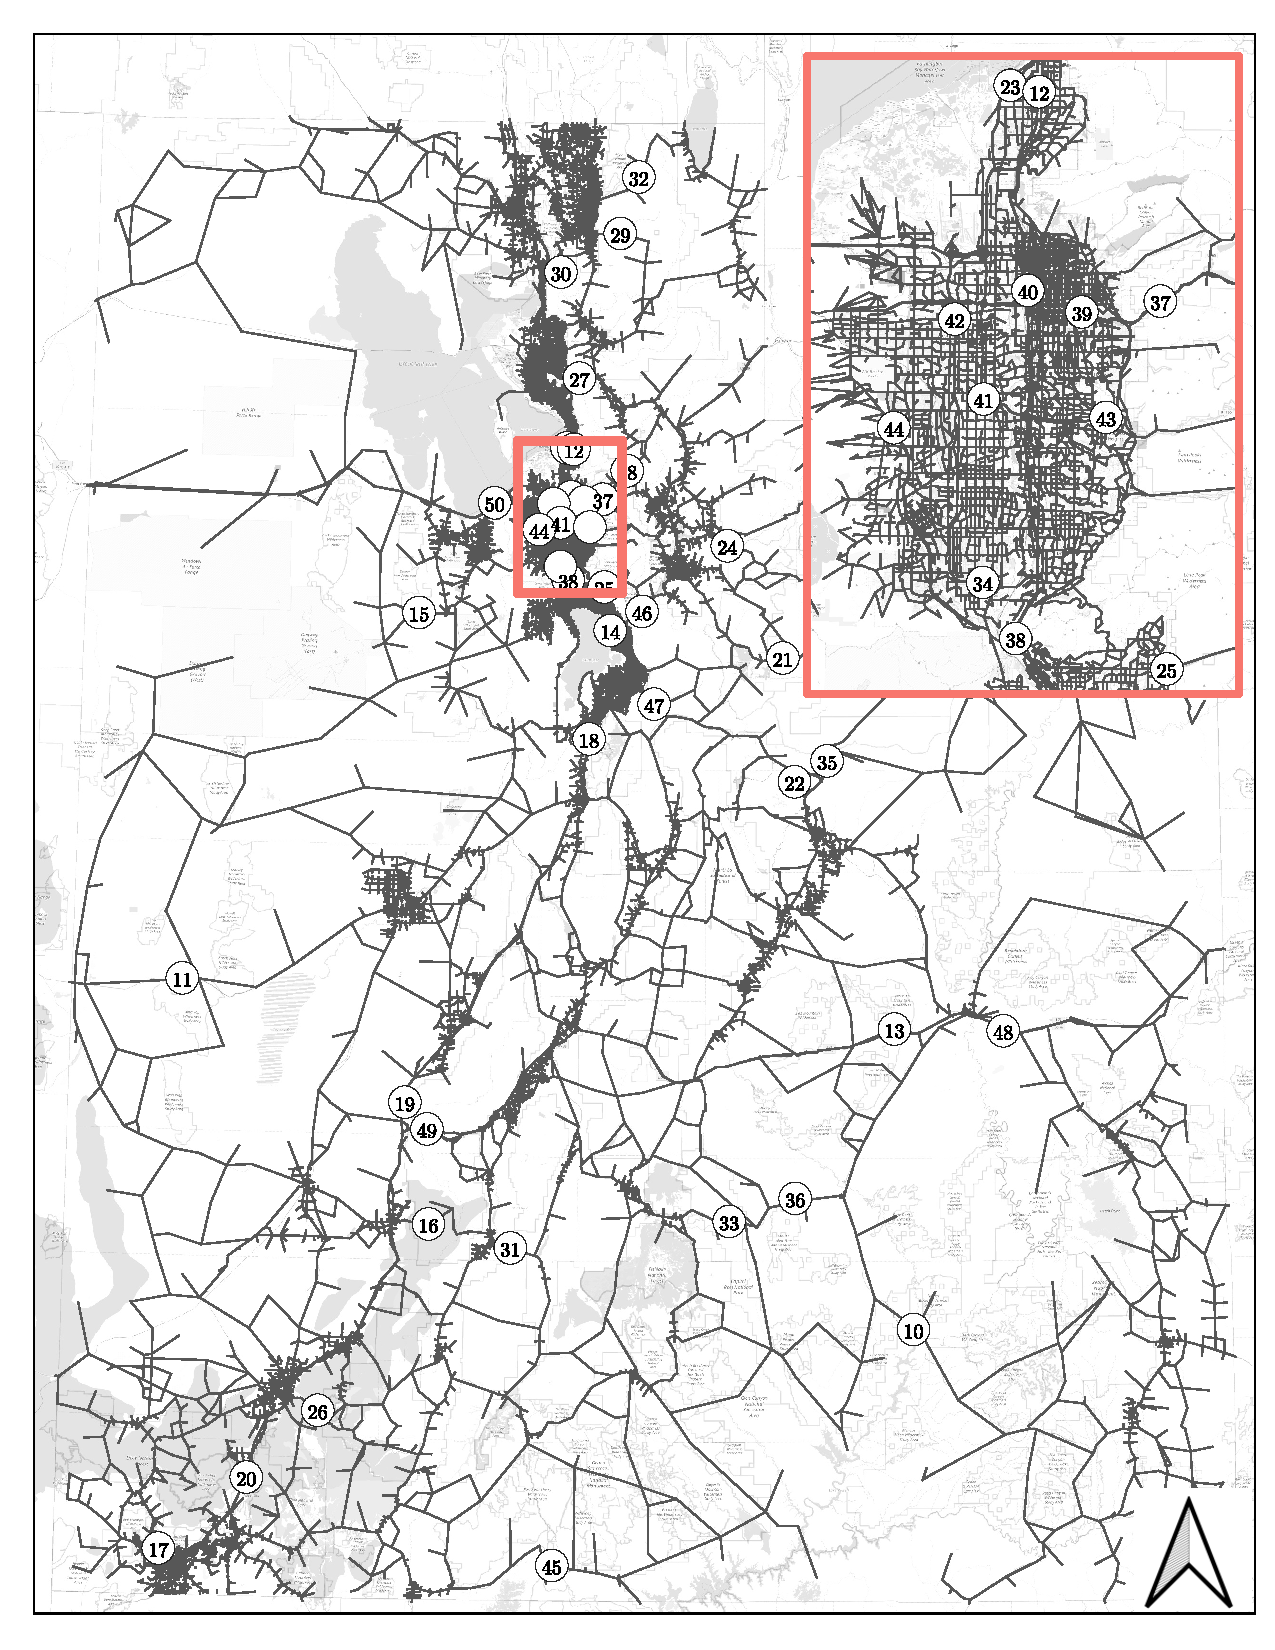
\includegraphics[width=0.75\linewidth]{figures/chapter4/resiliency_links_map.pdf}

}

\caption{Links Identified for Analysis.}\label{fig:linksmap}
\end{figure}

The following sections will present the results of the 41 scenarios analyzed. First,
Table \ref{tab:linktable} shows each of the scenarios we examined, labeled “road10”
for scenario 10, and “road11” for scenario 11. Other identifying information such as
route numbers or street names, and geographic or other identifying descriptions about
the locations where the link was cut are also provided.

\begin{table}

\caption{\label{tab:linktable}Link Table}
\centering
\begin{tabular}[t]{lll}
\toprule
LINK\_ID & ROUTE & LOCATION\\
\midrule
road10 & SR-95 & near Hite\\
road11 & US-6 & near King Top\\
road12 & I-15 & in Bountiful\\
road13 & I-70 & at Dragon Point (W of Green River)\\
road14 & I-15 & in Orem between Univ. Ave \& Center St\\
\addlinespace
road15 & SR-199 & near Rush Valley\\
road16 & SR-153 & between Beaver \& Junction\\
road17 & SR-18 & just North of St. George\\
road18 & I-15 & near Rocky Ridge (between Payson \& Nephi)\\
road19 & I-15 & near I-70 \& Filmore\\
\addlinespace
road20 & I-15 & near New Harmony\\
road21 & US-40 & East of Strawberry Reservoir\\
road22 & US-6 & in Carbon County North of Helper\\
road23 & Legacy Parkway & near West Bountiful\\
road24 & UT-35 & outside of Francis\\
\addlinespace
road25 & Timp Highway & at the base of AF Canyon\\
road26 & SR-14 & in Cedar Canyon\\
road27 & I-84 & between Ogden and Morgan\\
road28 & SR-65 & on the border of Salt Lake County \& Morgan County\\
road29 & SR-101 & East of Hyrum\\
\addlinespace
road30 & US-91 & between Brigham City \& Mantua\\
road31 & SR-62 & East of Kingston\\
road32 & US-89 & between Logan and Bear Lake\\
road33 & SR-24 & in Capitol Reef National Park\\
road34 & Bangerter & near Bluffdale\\
\addlinespace
road35 & SR-191 & between Helper \& Duchesne\\
road36 & SR-24 & near Steamboat Point\\
road37 & I-80 & in Parley's Canyon\\
road38 & I-15 & at the Point of the Mountain\\
road39 & I-80 & in SLC near Sugar House and 1300 E\\
\addlinespace
road40 & I-15 & in SLC between 2100 S \& 1300 S\\
road41 & I-215 & near Taylorsville\\
road42 & Bangerter & near West Valley City\\
road43 & I-215 & near Cottonwood Heights\\
road44 & MVC (UT-85) & West of West Jordan\\
\addlinespace
road45 & US-89 & near the Border of Arizona by Lake Powell\\
road46 & SR-189 & up Provo Canyon near Vivian Park\\
road47 & US-6 & up Spanish Fork Canyon near Diamond Fork Rd\\
road48 & I-70 & near Green River (NW of Moab)\\
road49 & I-70 & near Richfield \& Filmore\\
\addlinespace
road50 & I-80 & between SLC and Tooele\\
\bottomrule
\end{tabular}
\end{table}

\subsection{Link Rankings by Both Methods}
The logsum method results are as follows in Table \ref{linkresults}.
The results are ranked from the road with the largest (most positive
cost to the road with the smallest cost.

We can see that road 27, which corresponds to I-84 between Ogden and Morgan, experiences the largest cost per day according to the resiliency model. Following road 27, roads 50, 37, 30, and 17 make up the five most important roads according to the cost estimation provided by the resiliency model. Each of these roads with the exception of SR-18 in St. George, is an Interstate or State Highway facility in Northern Utah, which is heavily populated. Some roads, such as road 10, road 11, or road 33, which are located in remote parts of the state, experiences no measurable change to HBW, HBO, or NHB traffic. This is likely due to the location of the highway link that was cut. A ranking is provided for all of the roads in Table \ref{tab:linkresults}.

\begin{table}

\caption{\label{tab:linkresults}Link Analysis Results}
\centering
\begin{tabular}[t]{lrrll}
\toprule
Scenario & Delta & Cost Value & Route & Location\\
\midrule
ROAD27 & -23830.208 & 14893880.000 & I-84 & between Ogden and Morgan\\
ROAD50 & -19686.788 & 12304242.500 & I-80 & between SLC and Tooele\\
ROAD37 & -8932.691 & 5582931.875 & I-80 & in Parleys Canyon\\
ROAD30 & -7511.948 & 4694967.500 & US-91 & between Brigham City \& Mantua\\
ROAD17 & -5243.828 & 3277392.500 & SR-18 & just North of St. George\\
\addlinespace
ROAD46 & -4911.457 & 3069660.625 & SR-189 & up Provo Canyon near Vivian Park\\
ROAD38 & -4422.194 & 2763871.250 & I-15 & at the Point of the Mount\\
ROAD18 & -3186.967 & 1991854.375 & I-15 & in Rocky Ridge (between Payson \& Nephi)\\
ROAD42 & -2657.614 & 1661008.750 & Bangerter & near West Valley City\\
ROAD41 & -1700.167 & 1062604.375 & I-215 & near Taylorsville\\
\addlinespace
ROAD25 & -1139.020 & 711887.500 & Timp Highway & at the base of AF Canyon\\
ROAD24 & -387.467 & 242166.875 & UT-35 & outside of Francis\\
ROAD23 & -297.882 & 186176.250 & Legacy Parkway & near West Bountiful\\
ROAD20 & -253.712 & 158570.000 & I-15 & near New Harmony (between Cedar City \& St. George)\\
ROAD47 & -142.671 & 89169.375 & US-6 & up Spanish Fork Canyon near Diamond Fork Rd\\
\addlinespace
ROAD26 & -125.740 & 78587.500 & SR-14 & in Cedar Canyon\\
ROAD15 & -67.634 & 42271.250 & SR-199 & near Rush Valley\\
ROAD32 & -60.883 & 38051.875 & US-89 & between Logan and Bear Lake\\
ROAD14 & -45.386 & 28366.250 & I-15 & in Orem between Univ. Ave \& Center St\\
ROAD29 & -41.595 & 25996.875 & SR-101 & East of Hyrum\\
\addlinespace
ROAD31 & -40.108 & 25067.500 & SR-62 & East of Kingston\\
ROAD22 & -30.394 & 18996.250 & US-6 & in Carbon County North of Helper\\
ROAD49 & -17.768 & 11105.000 & I-70 & near Richfield \& Filmore\\
ROAD45 & -17.029 & 10643.125 & US-89 & near the Border of Arizona by Lake Powell\\
ROAD21 & -11.267 & 7041.875 & US-40 & East of Strawberry Reservoir\\
\addlinespace
ROAD36 & -10.170 & 6356.250 & SR-24 & near Steamboat Point\\
ROAD16 & -9.724 & 6077.500 & SR-153 & between Beaver \& Junction\\
ROAD48 & -9.717 & 6073.125 & I-70 & near Green River (NW of Moab)\\
ROAD19 & -7.623 & 4764.375 & I-15 & near I-70 \& Filmore\\
ROAD35 & -3.762 & 2351.250 & SR-191 & between Helper \& Dechesne\\
\addlinespace
ROAD13 & -0.135 & 84.375 & I-70 & at Dragon Point (W of Green River)\\
ROAD28 & -0.103 & 64.375 & SR-65 & on the border of Salt Lake County \& Morgan County\\
ROAD10 & 0.000 & 0.000 & SR-95 & near Hite\\
ROAD11 & 0.000 & 0.000 & US-6 & near King Top\\
ROAD33 & 0.000 & 0.000 & SR-24 & in Capitol Reef National Park\\
\addlinespace
ROAD12 & 894.999 & -559374.375 & I-15 & in Bountiful\\
ROAD44 & 2149.291 & -1343306.875 & MVC (UT-85) & West of West Jordan\\
ROAD43 & 4043.132 & -2526957.500 & I-215 & near Cottonwood Heights\\
ROAD40 & 5576.276 & -3485172.500 & I-15 & in SLC between 2100 S \& 1300 S\\
ROAD39 & 7434.744 & -4646715.000 & I-80 & in SLC near Sugar House and 1300 E\\
\addlinespace
ROAD34 & 9362.283 & -5851426.875 & Bangerter & near Bluffdale\\
\bottomrule
\end{tabular}
\end{table}

Table \ref{tab:timeresults} contains the ranking results from the travel
time method. Here, we see that the first five roads differ from the
results of the logsum model. Instead, road 48 becomes the most important
road due to costs experienced. Road 48 is a part of I-70 near Green River,
Utah. The other four roads that make up the top five most important roads
in the travel time method analysis are road 13, road 20, road 50, and road
49. Some of these roads appear in both the logsum and travel time methods.
Here again, several of the roads that are most important are located in
Northern Utah. It is important to note that the main driving factor as to
why a road was important or not in the travel time analysis was how much
freight and external traffic it experienced along that route. Including
the freight, even with the logsum results, changes the rankings
drastically because of the significantly higher value of time associated
with freight trips.

\begin{table}

\caption{\label{tab:timeresults}Travel Time Analsyis Results}
\centering
\begin{tabular}[t]{lrrrrrrrrrr}
\toprule
ROAD & IIF & XXF & IXF & HBW & HBO & NHB & REC & XXP & TIMEDIFF (Min) & Total Cost\\
\midrule
48 & 9.907799e+05 & 8.454694e+07 & 0.0217 & 195.8176 & 256.6567 & 28.9348 & 15447.5499 & 417991.5503 & 517790549.30 & 8.597164e+07\\
13 & 8.399095e+04 & 2.513068e+07 & 0.0000 & 0.0000 & 3.2527 & 0.0000 & 210.5181 & 95273.2859 & 76387376.42 & 2.531016e+07\\
20 & 5.685583e+05 & 1.871674e+07 & 175.0997 & 2873.2413 & 2640.2752 & 1208.8308 & 11372.0957 & 234813.5438 & 543606576.50 & 1.953838e+07\\
50 & 6.087866e+05 & 1.027499e+07 & 53.5297 & 244275.7151 & 108412.9438 & 84712.3575 & 398.7293 & 55870.1723 & 125766274.10 & 1.137750e+07\\
49 & 3.079064e+05 & 7.810609e+06 & 0.0000 & 78.0622 & 59.2752 & 17.6232 & 155.5550 & 29826.7738 & 62136743.99 & 8.148653e+06\\
\addlinespace
18 & 3.935367e+06 & 1.847822e+06 & 1148.1140 & 20436.1302 & 21163.5461 & 15362.6359 & 13839.5567 & 143890.3925 & 937282072.00 & 5.999030e+06\\
27 & 1.854494e+05 & 4.359448e+06 & 664.2652 & 35891.3868 & 20811.4770 & 52515.3604 & 207.6318 & 9608.6486 & 38255330.83 & 4.664596e+06\\
19 & 2.307693e+06 & 1.069414e+06 & 104.3208 & 67.2237 & 70.0649 & 13.2078 & 6829.1911 & 94820.4414 & 442572261.70 & 3.479012e+06\\
37 & 1.080281e+06 & 9.788824e+05 & 1127.7596 & 46220.2113 & 36178.1897 & 37631.6332 & 675.1268 & 5668.6435 & 51291892.31 & 2.186665e+06\\
47 & 1.411715e+06 & 6.163554e+05 & 8.1666 & 1631.6607 & 373.0056 & 468.6302 & 2600.3043 & 14011.5554 & 241897360.20 & 2.047164e+06\\
\addlinespace
38 & 1.341423e+06 & 3.911825e+05 & 153.2942 & 75916.0675 & 88791.1404 & 84969.5325 & 2485.9995 & 17292.8808 & 214931383.10 & 2.002214e+06\\
14 & 7.120600e+05 & 2.383607e+05 & 4.8294 & 31899.2443 & 35721.9390 & 38114.5497 & 1723.7055 & 10899.5483 & 134164459.50 & 1.068785e+06\\
30 & 9.099365e+05 & 8.036293e+02 & 514.7669 & 15379.0610 & 12882.8926 & 25635.9186 & 624.3483 & 3690.2614 & 115025954.80 & 9.694674e+05\\
39 & 1.681473e+05 & 6.624298e+05 & 297.8676 & 15712.6821 & 15091.4466 & 19512.5202 & 135.4998 & 2821.0313 & 8154310.12 & 8.841482e+05\\
22 & 4.217119e+05 & 2.608851e+05 & 7.9739 & 4.4674 & 27.9534 & 17.1794 & 1163.6510 & 4843.3492 & 83071865.27 & 6.886616e+05\\
\addlinespace
45 & 8.637883e+02 & 5.509410e+05 & 145.7363 & 183.9739 & 232.6245 & 78.5503 & 13.4424 & 40330.4295 & 5447581.96 & 5.927895e+05\\
21 & 5.378431e+05 & 0.000000e+00 & 0.3000 & 26.3054 & 89.7595 & 38.6124 & 422.8649 & 3397.7307 & 34192023.06 & 5.418187e+05\\
40 & 2.662065e+05 & 1.040071e+05 & 1.0558 & 19182.8100 & 19129.6986 & 20511.6397 & 266.8174 & 3233.3472 & 35243767.20 & 4.325389e+05\\
12 & 2.993304e+05 & 7.818270e+04 & 0.1602 & 12585.8118 & 9574.6810 & 12507.6326 & 251.2141 & 3445.9185 & 38335415.98 & 4.158785e+05\\
35 & 1.812866e+05 & 0.000000e+00 & 0.0000 & 16.8416 & 69.7900 & 1.0298 & 355.1579 & 2691.0964 & 65228930.22 & 1.844205e+05\\
\addlinespace
46 & 8.059370e+04 & 1.041404e+03 & 99.7032 & 15111.9443 & 21009.6172 & 12684.3356 & 924.3246 & 171.8691 & 78989455.18 & 1.316369e+05\\
41 & 1.515385e+04 & 0.000000e+00 & 0.4593 & 11092.2455 & 17748.7203 & 22620.5138 & 44.2187 & 0.0000 & 1280460.38 & 6.666000e+04\\
34 & 1.951111e+04 & 0.000000e+00 & 0.2150 & 8202.9795 & 11805.6401 & 14453.2904 & 57.3198 & 0.0000 & 3104087.28 & 5.403055e+04\\
32 & 4.771497e+04 & 8.089437e+02 & 0.9723 & 736.0051 & 596.8124 & 124.5756 & 5.3209 & 0.0000 & 16516731.75 & 4.998760e+04\\
43 & 4.898116e+03 & 0.000000e+00 & 32.3321 & 6214.8820 & 10069.7932 & 13886.2694 & 84.3510 & 0.0000 & 1061412.27 & 3.518574e+04\\
\addlinespace
16 & 3.053316e+04 & 0.000000e+00 & 0.1102 & 35.2392 & 0.8310 & 30.9960 & 118.4095 & 0.0000 & 400528.31 & 3.071875e+04\\
42 & 4.319564e+03 & 0.000000e+00 & 1.0689 & 6623.8202 & 3955.9950 & 4711.9401 & 0.9951 & 0.0000 & 118983.58 & 1.961338e+04\\
17 & 2.085366e+03 & 0.000000e+00 & 0.1453 & 2384.3859 & 3350.5890 & 6416.1449 & 1.4531 & 0.0000 & 2714732.79 & 1.423808e+04\\
44 & 3.495956e+03 & 0.000000e+00 & 0.0112 & 3577.6774 & 1909.6427 & 5214.1316 & 2.3779 & 0.0000 & 272105.44 & 1.419980e+04\\
11 & 7.576949e+03 & 0.000000e+00 & 0.0000 & 0.0206 & 2.7587 & 0.0505 & 0.5076 & 0.0000 & 5602443.84 & 7.580286e+03\\
\addlinespace
24 & 1.884429e+03 & 0.000000e+00 & 0.0000 & 847.0520 & 276.3691 & 1828.9714 & 0.6032 & 0.0000 & 4099829.14 & 4.837425e+03\\
33 & 4.088993e+03 & 0.000000e+00 & 0.0479 & 2.6681 & 4.8372 & 0.0000 & 23.9748 & 0.0000 & 2698368.92 & 4.120521e+03\\
25 & 5.627087e+01 & 0.000000e+00 & 0.0000 & 516.3094 & 272.7545 & 1852.3708 & 0.2881 & 0.0000 & 66958.96 & 2.697994e+03\\
36 & 1.920113e+03 & 0.000000e+00 & 0.0000 & 12.8155 & 33.8723 & 12.5058 & 17.9324 & 0.0000 & 1826834.26 & 1.997239e+03\\
26 & 7.331829e+02 & 0.000000e+00 & 0.0779 & 261.0639 & 214.9443 & 189.3878 & 18.4149 & 0.0000 & 978315.43 & 1.417072e+03\\
\addlinespace
31 & 2.595082e+02 & 0.000000e+00 & 0.0000 & 324.7364 & 482.7504 & 157.8675 & 0.5736 & 0.0000 & 2192510.85 & 1.225436e+03\\
10 & 3.459434e+02 & 0.000000e+00 & 0.0000 & 0.0000 & 0.0000 & 0.0000 & 780.4662 & 0.0000 & 4755463.02 & 1.126410e+03\\
15 & 2.097366e+02 & 0.000000e+00 & 0.0032 & 221.0662 & 258.3935 & 67.3873 & 4.4245 & 0.0000 & 1160411.30 & 7.610113e+02\\
23 & 1.682285e+02 & 0.000000e+00 & 0.0026 & 84.6450 & 52.9403 & 123.9602 & 0.0107 & 0.0000 & 13581.54 & 4.297873e+02\\
29 & 1.928357e+00 & 0.000000e+00 & 0.0058 & 122.3929 & 0.3114 & 62.3210 & 0.0000 & 0.0000 & 373344.59 & 1.869595e+02\\
\addlinespace
28 & 5.780939e+00 & 0.000000e+00 & 0.0000 & 0.0239 & 0.0477 & 0.0636 & 12.8707 & 0.0000 & 55504.21 & 1.878684e+01\\
Base & 0.000000e+00 & 0.000000e+00 & 0.0000 & 0.0000 & 0.0000 & 0.0000 & 0.0000 & 0.0000 & 0.00 & 0.000000e+00\\
\bottomrule
\end{tabular}
\end{table}

Some other interesting findings are that in the top 10 of each analysis
methods, three scenarios appear in both rankings. Road 50, which
corresponds to I-80 between Tooele and SLC, road 27 which corresponds to I-
84 in Weber Canyon, road 37 which corresponds to I-80 in Parley’s Canyon,
and road 27 which is I-84 between Ogden and Morgan, are included in the
top 10 scenarios for both methods of analysis. This is likely due to the
number of passenger trips along these routes and the number of freight
trips that occur along these routes as well. Several of these routes are
the only way through mountain ranges in the routes geographic location.

\subsection{Positive Benefit Scenarios}

Five of the scenarios indicated a benefit resulting from highway link closure. These scenarios were examined more closely to determine what possible causes could exist beghind these atypical and unexpected results. The affected links are all located in Salt Lake Valley area at the following locations: Bangerter Highway near Bluffdale, I-80 near 1300 E, I-15 between 2100 S and 1300 S, I-215 near Cottonwood Heights, Mountain View Corridor near West Jordan and I-15 near Bountiful.

It was determined that a likely cause which explains these atypical r
esults is that the shortest path by time is not the shortest path by
distance. The automobile accessibility is determined by the AM congested
travel time in the Utah Statewide Travel Model (USTM). The travel distance
– used to determine the accessibility of destinations by driving or
walking – is the distance of that path, and not the actual shortest
distance path as might be more preferable. Additionally, it was found that
the alternative route between Grouse Creek, UT and SLC, the alternative
route was nearly twice as long in the case where I-80 was closed between
Toeele and Salt Lake. This discovery led us to understand that not all
route chocies become logical when made using only the model data. In
reality, it is much more likely that a user would find a shorter route
which consists of roads that are not all in the state highway system.

Another discovery we made, is that When a highway link is broken, the new
shortest path by time is longer than in the base scenario with this link
available. But the new path may actually be shorter by distance. This
causes an increase in the utility of accessing destinations by non-
motorized modes, potentially overwhelming the decrease in automobile
utility.

This occurence is only observed in heavily urbanized regions for two reasons:
\begin{itemize}
	\item The presence of high-speed expressways and parallel local roads
  means that alternate paths with shorter distances but longer vehicle
  times are more likely.
	\item The increased availability of destinations within the non-
  motorized distance threshold (50 miles) means that alternative
  destinations exist.
\end{itemize}

Overall, the results of the analysis indicate that the likely cause of a
positive cost being estimated for these five scenarios is that there are
easily
accessible alternate routes in the area, or extremely different alternate
routes along with competing TAZ of similar size in the DC size term
equation.

\section{Summary}

The overall results show that the resiliency model is more sensitive to
network changes than the travel time comparison. The ability for a user to
choose both a mode and destination (or alternate destination) cause the
logsum results to often estimate a smaller cost than the travel time
results would. However, when the travel time results are factored in, the
overall rankings of the 41 scenarios considered change dramatically. This
is due to the large expenses experienced by freight traffic, which has a
much higher VOT than other passenger trips do. In summary, Table
\ref{tab:linkresults} and Table \ref{tab:timeresults} show the rankings
for both the logsum and travel time analysis methods respectively. The
logsum suggests that I-84 between Ogden and Morgan is the most important
road, while the travel time method, or total priority, indicates that I-70
near Green River is the most important road due to cost associated with
closure.
